\documentclass[xcolor=table]{beamer}

\usepackage{booktabs}
\usepackage{hyperref}
\usepackage[table]{xcolor}
\usepackage{tikz}
\usepackage{graphics}
\usetikzlibrary{calc}

\setbeamertemplate{navigation symbols}{}%remove navigation symbols

\title{Subgame Perfection}
\subtitle{Game Theory}
\author{Vincent Knight}
\date{}

\tikzstyle{level 1}=[level distance=3.5cm, sibling distance=3.5cm]
\tikzstyle{level 2}=[level distance=3.5cm, sibling distance=2cm]
\tikzstyle{player} = [text width=4em, draw, text centered, rectangle, fill=blue!20, inner sep=1pt]
\tikzstyle{nature} = [minimum width=3pt,circle,  draw, fill=red!20, inner sep=1pt]
\tikzstyle{end} = [circle, minimum width=3pt, fill, inner sep=0pt, right]
\tikzstyle{dot} = [draw,shape=circle,fill=blue]

\begin{document}

\frame{\titlepage}

\frame{
\tikzstyle{level 1}=[level distance=2.5cm, sibling distance=3.5cm]
\tikzstyle{level 2}=[level distance=2.5cm, sibling distance=2cm]
\tikzstyle{level 3}=[level distance=2.5cm, sibling distance=1cm]
\tikzstyle{player} = [text width=5em, draw, text centered, rectangle, fill=blue!20, inner sep=1pt]
\tikzstyle{nature} = [minimum width=3pt,circle,  draw, fill=red!20, inner sep=1pt]
\tikzstyle{end} = [circle, minimum width=3pt, fill, inner sep=0pt, right]
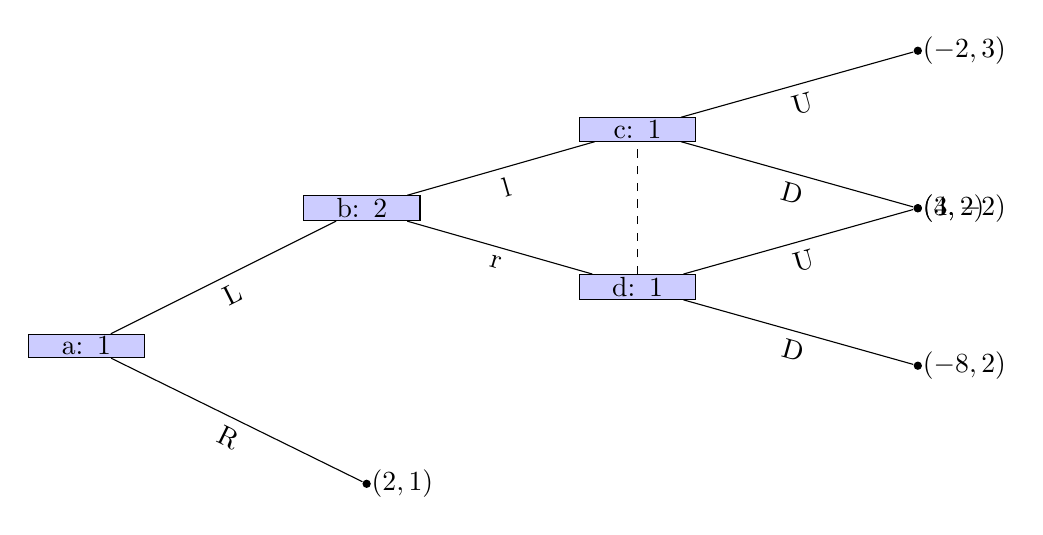
\begin{tikzpicture}[grow=right, sloped]
    \node[player]{a: 1}
        child {node[end] {} node[right] {$(2,1)$} edge from parent node[below] {R}}
        child {node[player] {b: 2}
                child {node (A) [player] {d: 1}
                    child {node[end] {} node [right] {$(-8,2)$} edge from parent node[below] {D}}
                    child {node[end] {} node [right] {$(3,-2)$} edge from parent node[below] {U}}
                        edge from parent node[below] {r}}
                child {node (B) [player] {c: 1}
                child{node[end] {} node[right]{$(4,2)$} edge from parent node[below]{D}}
                child{node[end] {} node[right]{$(-2,3)$} edge from parent node[below]{U}} edge from parent node[below] {l}} edge from parent node[below] {L}};
        \draw [dashed] (A) -- (B);
\end{tikzpicture}

\pause
$$S_1=\{LU,LD,RU,RD\}\;\;S_2=\{l,r\}$$
}

\frame{
$$S_1=\{LU,LD,RU,RD\}\;\;S_2=\{l,r\}$$
$$
\begin{pmatrix}
(-2,3)&(3,-2)\\
(4,2)&(-8,3)\\
(2,1)&(2,1)\\
(2,1)&(2,1)\\
\end{pmatrix}
$$
\pause
\begin{center}
Nash Equilibrium: $(LD,l)$
\end{center}
}

\frame{
\begin{itemize}
\item \textbf{Subgame:} In an extensive form game, a node x is said to initiate a subgame if and only if $x$ and all successors of x are in information sets containing only successors of $x$.
\item \textbf{Subgame perfect equilibria:} A subgame perfect Nash equilibrium is a Nash equilibrium in which the strategy profiles specify Nash equilibria for every subgame of the game.
\end{itemize}
}

\frame{
\tikzstyle{level 1}=[level distance=2.5cm, sibling distance=3.5cm]
\tikzstyle{level 2}=[level distance=2.5cm, sibling distance=2cm]
\tikzstyle{level 3}=[level distance=2.5cm, sibling distance=1cm]
\tikzstyle{player} = [text width=5em, draw, text centered, rectangle, fill=blue!20, inner sep=1pt]
\tikzstyle{nature} = [minimum width=3pt,circle,  draw, fill=red!20, inner sep=1pt]
\tikzstyle{end} = [circle, minimum width=3pt, fill, inner sep=0pt, right]
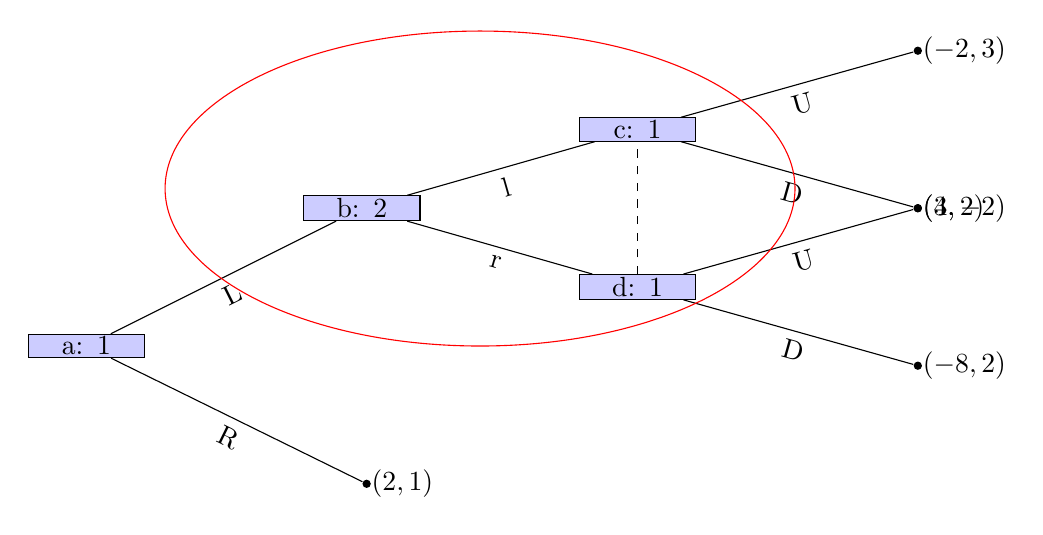
\begin{tikzpicture}[grow=right, sloped]
    \node[player]{a: 1}
        child {node[end] {} node[right] {$(2,1)$} edge from parent node[below] {R}}
        child {node[player] {b: 2}
                child {node (A) [player] {d: 1}
                    child {node[end] {} node [right] {$(-8,2)$} edge from parent node[below] {D}}
                    child {node[end] {} node [right] {$(3,-2)$} edge from parent node[below] {U}}
                        edge from parent node[below] {r}}
                child {node (B) [player] {c: 1}
                child{node[end] {} node[right]{$(4,2)$} edge from parent node[below]{D}}
                child{node[end] {} node[right]{$(-2,3)$} edge from parent node[below]{U}} edge from parent node[below] {l}} edge from parent node[below] {L}};
        \draw [dashed] (A) -- (B);
        \pause
        \draw [red] (5,2) ellipse (4cm and 2cm);
\end{tikzpicture}

\onslide<2>{
\begin{center}
Nash Equilibrium: $(LD,l)$ \hspace{2cm}  $\begin{pmatrix}(-2,3)&(3,-2)\\(4,2)&(-8,2)\end{pmatrix}$
\end{center}}
}

\end{document}
